\documentclass[11pt,a4paper,twoside,pdftex]{book}

\usepackage[T1]{fontenc}
%\usepackage{ae,aecompl,aeguill}
\usepackage{times}
\usepackage[pdftex]{graphicx}
\usepackage[linkcolor=blue]{hyperref}
\usepackage{relsize,fancyvrb}

\usepackage{eso-pic}
\newcommand\BackgroundPic{
\put(0,0){
\parbox[b][\paperheight]{\paperwidth}{%
\vfill
\centering
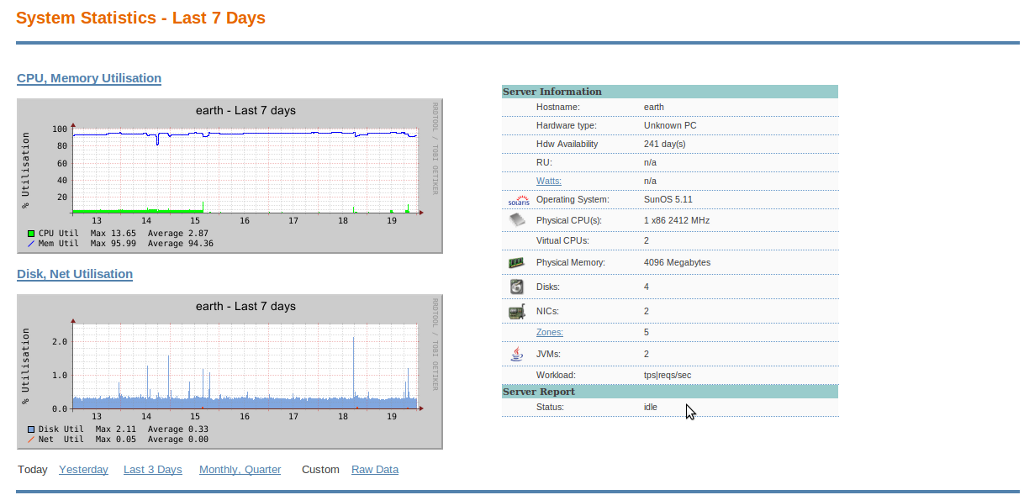
\includegraphics[width=\paperwidth,height=\paperheight,
keepaspectratio]{back.png}%
\vfill
}}}


% generates the chapter header
\usepackage[Lenny]{fncychap}


% generates the chapter header
%\usepackage[avantgarde]{quotchap}
%\renewcommand\chapterheadstartvskip
%              {\vspace*{-5\baselineskip}}
%\usepackage{helvet}
%\renewcommand\sectfont{\sffamily\bfseries}


% generates the frontpage
\makeatletter
\def\thickhrulefill{\leavevmode \leaders \hrule height 1pt\hfill \kern \z@}
\renewcommand{\maketitle}{\begin{titlepage}%
    \let\footnotesize\small
    \let\footnoterule\relax
    \parindent \z@
    \reset@font
    \null
    \vskip 10\p@
    \hbox{\mbox{%
        \hspace{4pt}%
        
\includegraphics[keepaspectratio]{sdrnew40x42.png}
        \hspace{4pt}
        }%
      \vrule depth 0.9\textheight%
      \mbox{\hspace{2em}}
      \vtop{% %%%%%%%%%%%%%%%%%%
        %\vskip 40\p@
        \vskip 240\p@
        \begin{flushleft}
          \Large \bfseries \@author \par
        \end{flushleft}
        %\vskip 80\p@
        \vskip 40\p@
        \begin{flushleft}
          \huge \bfseries \@title \par
          \Large \bfseries ver 0.71 \par
        \end{flushleft}
        \vfil
        }}
    \null
  \end{titlepage}%
  \setcounter{footnote}{0}%
}
\makeatother


% marginal notes
\newcommand\marginlabel[1]{\mbox{}\marginpar
  {\raggedright\hspace{0pt}#1}}



% sets title, author, date
\title{System Data Recorder \\
       User Guide}
\author{www.systemdatarecorder.org}
\date{December 28, 2009}

 
% sets the PDF info
\pdfinfo{
   /Author (sparvu)
   /Title  (User Guide)
   % YYYYMMDDHHmmss
   /CreationDate (D:20091129120000)
   /Subject (SDR Installation)
   /Keywords (SDR;Install;Unix)
}


% %%%%%%%%%%%%%% %
% Begin Document %
% %%%%%%%%%%%%%% %
\newbox\bwk\edef\tempd#1pt{#1\string p\string t}\tempd\def\nbextr#1pt{#1}
\def\npts#1{\expandafter\nbextr\the#1\space}
\def\ttwplink#1#2{\special{ps:1 0 0 setrgbcolor}#2\special{ps:0 0 0 setrgbcolor}\setbox\bwk=\hbox{#2}\special{ps:( linkto #1)\space\npts{\wd\bwk} \npts{\dp\bwk} -\npts{\ht\bwk} true\space Cpos}}
\begin{document}

\frontmatter
\maketitle
\pagebreak
\begin{small}

\noindent
Copyright \copyright 2005-2012 Stefan Parvu and Contributers. All rights reserved.
\\

\noindent
This document is free; you can redistribute it and/or modify it
under the terms of the GNU General Public License as published by
the Free Software Foundation; either version 2 of the License, or
(at your option) any later version.

\noindent
\newline
This document is distributed in the hope that it will be useful, but
WITHOUT ANY WARRANTY; without even the implied warranty of
MERCHANTABILITY or FITNESS FOR A PARTICULAR PURPOSE\@.  See the GNU
General Public License for more details.

\noindent
\newline
You should have received a copy of the GNU General Public License
along with this document; if not, write to the Free Software
Foundation, Inc., 675 Mass Ave, Cambridge, MA 02139, USA.
(http://www.gnu.org/copyleft/gpl.html)

\end{small}

\endinput


\chapter*{Credits}

\noindent
System Data Recorder is an open source project, started late 2005,
to provide standard server infrastructure performance monitoring for 
Linux and Solaris based systems.

\noindent
\newline
Some ideas went into SDR as a frustration using other types of performance 
monitoring systems, some other simple ended up as being important and useful. 
During 2007 concepts from Guerrilla Capacity Planning of Dr. Neil Gunther made 
ground rules for future SDR versions.

\noindent
Many people contributed ideas, suggestions over the time. To all contributors, 
many thanks, for your support !

\noindent
\newline
Finally, thanks to LATEX community for keeping alive the project over the years.
The current manual has been prepared using the professional \LaTeX{} document 
processing system.

\endinput

\tableofcontents
%\AddToShipoutPicture*{\BackgroundPic}
%\listoffigures
%\listoftables

\mainmatter
% Include Chapters

% Chapter 1

\chapter{Introduction}

\noindent
After more than 25 years of computer business we still lack consistent 
performance monitoring between different operating systems, each system 
deploying its own type of monitoring and data collection. This makes difficult 
to have consistent data collection over long periods of time, from
different systems. There were some efforts, for example the Universal Measurement 
Architecture project, started by OpenGroup in 1997 which was trying to 
standardize the performance measurement process. Majority of the computer 
vendors found this not important and with no financial returns 
the project failed and unfortunately nothing came up as a final solution.

\bigskip
\noindent
Today, the majority of IT companies require you to buy or download a 
separately software which records and stores data from different 
operating systems and applications. Each of these applications 
store and keep data different from vendor to vendor. Some 
use a relational database management system to save all collected data.
Some other use dedicated types of databases like RRDtool or proprietary 
systems where all data is saved and stored over periods of time. 
In addition, these applications include extra modules on top of system 
recording: event and alert management, inventory, application monitoring 
and profiling. This way such systems turn big, complex and hard to 
understand.

If we step back and we look other industries, how are they doing it, 
we see a completely different picture.

\begin{enumerate}
\item Aerospace industry: FDR. Airplanes for examples use some sort of 
recorders, usually found as a device called flight data recorder FDR, 
used to store aircraft data parameters. Such unit is found by default 
on many airplanes nowadays and its usage is regulated by governments and 
federal administrations, example FAA in United States. This device sometimes
is referred as the black box.

\item Shipbuilding industry: VDR. Ships, boats or other type of vessels 
use some sort of recorder, called voyager data recorder VDR, used to 
store vessel data parameters. Similar to aerospace industry such devices 
are required when a certain vessel must comply with international 
standards, example International Convention for the Safety of Life 
at Sea, SOLAS. Used mainly for accident investigation the VDR can serve 
as preventive maintenance, performance efficiency monitoring, heavy weather 
damage analysis, accident avoidance and training purposes to improve 
safety and reduce running costs. This device sometimes is referred as the 
black box.

\item Auto industry: EDR. Automobiles use some sort of device used to store 
vehicle parameters, called event data recorder EDR. Again such devices can 
serve as the main source for accident investigations. EDRs are not enforced 
by any standard organizations and are not really required by law so their 
usage varies from vendor to vendor. National Highway Traffic Safety 
Administration NHTSA proposed a series of changes to standardize and enforce 
mandatory EDR installation and usage by vendors. Around 2010 over 
85\% of all vehicles in US would already have some sort of EDR installed.

\item Computer industry: None. Computers, mainframes, servers or workstations 
have no such recording devices installed. Manufacturers are not interested in 
standardizing this effort since they prefer selling additional software 
packages which can perform such recording features for an extra cost. 
The lack of standardization and agreements between vendors resulted 
in a complete different picture than other industries. Currently, there are 
houndreads of performance monitoring solutions for computer systems.
\end{enumerate}

\bigskip
\noindent
What if we try to adopt what other industries are using and define 
a number of standard recorders, found on each computer system, 
no matter if that is a database or application server. And what if we use 
same way no matter what the operating system really is, wouldn't this be great ?

System Data Recorder, shortly SDR, is trying to offer some help here. Such
recorders, data collectors can be delivered as part of the operating system, 
making uniform the process of collection and analysis between operating 
systems. The collected raw data would be similar between operating systems 
and would help the analysis process. This is in general possible for any 
UNIX systems which are similar with each other, since all are POSIX systems 
and follow similar industry standards, like The Open Group. 

\begin{figure}[!ht]
\centering
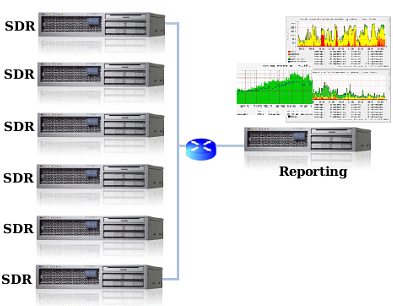
\includegraphics[width=80mm,height=60mm]{sdr-schema1.png}
\caption{SDR Recording/Reporting}
\label{fig:sdr-schema1}
\end{figure}

\bigskip
\noindent
There are four main recorders: sysrec, cpurec, nicrec, diskrec. 
Each recorder runs as a separate Perl5 process without any relation 
to the others. This makes very flexible to operation mode of all recorders, 
since they are autonomous. Additional there are different other recorders 
which can collect other type of system or application data: 
netrec, jvmrec, hdwrec, webrec. 

\noindent
All recorded data is stored as plain ASCII data, easy to be accessed by any 
3rd party system or other applications. The main idea is to have the data 
collection process standard between operating systems: Solaris, Linux, BSD. 

\bigskip
\noindent
The second module of SDR, the Reporting module, consists of several key
technologies: Round Robin Database Tool RRDtool, Perl 5, R Statistical Language, 
PDQ analytical solver all running on top of a HTTP server. All these coupled
with some visualization utilities makes SDR Reporting easy to be used in 
understanding the workloads running on a certain hardware infrastructure.

\endinput


% Release Notes
\include{chapter2}

% Installation
\include{chapter3}
 %  Requirements
 %  Install phase
 %  Start
 
\backmatter
\end{document}
% %%%%%%%%%%%%%% %

